\documentclass[12pt, aspectratio=169]{beamer}   %default is 11pt
%aspectratio sets the ratio of frame{16:9}
\usetheme[progressbar=frametitle]{metropolis}
\usepackage{color, amsmath, appendixnumberbeamer, ragged2e, booktabs, pgfplots, caption, xspace, hyperref, graphicx, subfigure}
\setbeamercolor{frametitle}{fg=black, bg=white}
\usepackage[scale=2]{ccicons}
\usepgfplotslibrary{dateplot}
\newcommand{\themename}{\textbf{\textsc{metropolis}}\xspace}
\usepackage[export]{adjustbox}
\usepackage[utf8]{inputenc}
\usepackage[dvipsnames]{xcolor}
\usepackage{multicol, multirow}

%\setbeamertemplate{navigation symbols}{}  %hides navigation buttons at the bottom.
\setbeamercovered{transparent}
\setbeamertemplate{headline}{} %hides headlines
\setbeamercovered{transparent}

\usepackage[backend=bibtex, style=authoryear]{biblatex}
\addbibresource{Bibliography.bib}

\title[Shale Gas Shock and Education Decisions]{Dutch Disease or Dutch Blessing?\\ Shale Gas Shock and Education Decisions\\ {\footnotesize (preliminary draft)}}
\author[Wooyong Park]{Wooyong Park}
\institute{Stanford Graduate School of Business}
\date{\today}

% \setbeamertemplate{footline}{%
%   \leavevmode%
%   \hbox{%
%     \begin{beamercolorbox}[wd=.5\paperwidth,ht=2.5ex,dp=1ex,center]{author in head/foot}%
%       \usebeamerfont{author in head/foot}\insertshortauthor
%     \end{beamercolorbox}%

%     \begin{beamercolorbox}[wd=.5\paperwidth,ht=2.5ex,dp=1ex,right]{date in head/foot}%
%       \usebeamerfont{date in head/foot}\insertshorttitle\hspace*{2em}%
%       \insertframenumber{} / \inserttotalframenumber\hspace*{2ex}%
%     \end{beamercolorbox}%
%   }%
%   \vskip0pt%
% }

\definecolor{lightgray}{RGB}{230, 230, 230}
\definecolor{lightgrey}{RGB}{200, 200, 200}

% Customize alertblock colors
\setbeamercolor{block title alerted}{bg=lightgrey, fg=black}
\setbeamercolor{block body alerted}{bg=lightgray, fg=black}

%----------------------------------------------------------------------------------------
%    PRESENTATION SLIDES
%----------------------------------------------------------------------------------------

\begin{document}
\begin{frame}
    % Print the title page as the first slide
    \titlepage
\end{frame}

\begin{frame}{Contents}
    \tableofcontents
\end{frame}

%------------------------------------------------
\section{Introduction}

\begin{frame}{Motivation}

\begin{itemize}
    \item \textbf{Dutch Disease}  refers to the reallocation of resources from capital-intensive sectors to booming resource-based sectors, which hinders the growth of the former and increases the region’s or country’s dependence on natural resources.
   \begin{itemize}
        \item Consistent with classical trade theory (Rybczynski Theorem), existing empirical research has primarily focused on developing economies.
        \item also related to \textbf{educational decisions}, since capital-intensive sectors typically require more education than resource-based sectors
    \end{itemize}
    \item The massive \textbf{shale gas discoveries} in the 2000s, centered around the Barnett basin (TX) and the Marcellus basin (PA), provide a compelling setting for testing this theory in a developed economy context.
\end{itemize}
\end{frame}
%------------------------------------------------
\begin{frame}{Goals}

\begin{itemize}
    \item[] \textbf{\large Empirical Side}
    \begin{itemize}
        \item Based on \textcite{sun_estimating_2021}, provide \textit{inter-state} comparisons on the impact of the shale gas shock on three key variables: \textbf{household income}, \textbf{high school attendance}, and \textbf{college decisions}.
        \item It investigates heterogeneity in these effects (mainly across different income levels).
    \end{itemize}

    \vfill

    \item[] \textbf{\large Econometric Side}
    \begin{itemize}
        \item assess the heterogeneity in a more data-driven way(\cite{athey2016recursive}), extending R-learners(\cite{wager2018estimation}) to a panel or a repeated cross-section framework
    \end{itemize}
\end{itemize}

\end{frame}

%------------------------------------------------
% 3. Literature Review
\begin{frame}{Literature Review}
\begin{itemize}
    \item Positive Effects of Shale Gas Shock \textbf{on Income}
    \begin{itemize}
        \item Higher per capita income in shale counties(\cite{weinstein2011economic})
    \end{itemize}
    
    \item Negative Effects of Shale Gas Shock \textbf{on Education}
    \begin{itemize}
        \item Decline in high school and college attainment in West Virginia, Montana, and North Dakota(\cite{rickman2017shale})
        \item Increased dropout rates among immigrants in Texas(\cite{carpenter2019texas})
    \end{itemize}
    
    \item Limitations in Prior Studies and our Contribution
    \begin{itemize}
        \item Not much discussions of \textbf{heterogeneous treatment effects}
        \item Mostly intra-state county-level comparisons, inter-state comparisons rely on SCMs(\cite{abadie2010synthetic})
    \end{itemize}
\end{itemize}
\end{frame}
%------------------------------------------------
\section{Empirical Strategy}
\begin{frame}{IPUMS ACS Data}
    \footnotesize
    \begin{itemize}
        \item IPUMS ACS - 1yr from 2000 to 2010
        \item Variables of Interest : Household Income, Education Attainment, School Attendance, etc.
        \item  excluded five states {\tiny  (Hawaii, Alaska, Puerto Rico, Colorado, and Wyoming)}
        \item Covariates are mostly balanced, but shale states tend to have lower income (documented widely in prev. research)
    \end{itemize}
\begin{table}[ht]
\centering
\tiny
\begin{tabular}{l|l||c|ccc|ccc}
 \hline
 & Age & Observations & \multicolumn{3}{c|}{Family Income} & \multicolumn{3}{c}{Education (Years)} \\
 & & & Mean & Std. Dev. & Count & Mean & Std. Dev. & Count \\
 \hline
 \multirow{4}{*}{Non-shale} & [5, 10] & 1,308,465.00 & 72,838.58 & 75,229.40 & 1,298,525.00 & 0.63 & 1.31 & 1,308,465.00 \\
 & [16, 18] & 716,276.00 & 76,209.93 & 75,288.26 & 684,920.00 & 10.60 & 1.32 & 716,276.00 \\
 & [18, 24] & 1,396,758.00 & 59,542.08 & 63,236.34 & 1,287,939.00 & 12.37 & 2.02 & 1,396,758.00 \\
 & total & 17,029,516.00 & 71,707.67 & 72,064.18 & 16,680,293.00 & 11.14 & 5.28 & 16,429,863.00 \\
 \multirow{4}{*}{Shale} & [5, 10] & 301,477.00 & 62,547.86 & 64,017.72 & 299,038.00 & 0.60 & 1.25 & 301,477.00 \\
 & [16, 18] & 162,607.00 & 67,489.58 & 66,903.25 & 155,650.00 & 10.48 & 1.40 & 162,607.00 \\
 & [18, 24] & 315,031.00 & 52,141.72 & 55,290.96 & 291,304.00 & 12.22 & 2.00 & 315,031.00 \\
 & total & 3,794,579.00 & 63,292.86 & 62,940.60 & 3,709,749.00 & 10.74 & 5.21 & 3,656,064.00 \\
 \hline
\end{tabular}
\caption{Summary Statistics(Mean and SD weighted)}
\label{tab:sum_stat}
\end{table}
\end{frame}
%------------------------------------------------


\begin{frame}{Methodology - \textcite{sun_estimating_2021} DiD}

    \begin{columns}
    \column{0.47\linewidth}
\begin{table}[htbp]
    \centering
    \begin{tabular}{c| c}
        
        Year & State \\
        \hline \hline
        2005 & Texas \\
        2006 & Arkansas \\
        2006 & Oklahoma \\
        2008 & Alabama \\
        2008 & Louisiana \\
        2008 & Pennsylvania \\
        2008 & West Virginia \\
    \end{tabular}
    \caption{\footnotesize Shale Gas Extraction Beginnings}
    \label{tab:shale-gas-extraction}
\end{table}
    \column{0.06\linewidth}
    \centering
    \Huge
    =
    \column{0.47\linewidth}
    \begin{table}[h]
        \centering
        \footnotesize
        \begin{tabular}{|c|c|c|c|c|c|}
        \hline
             &$t_1$&$t_2$&$t_3$&$t_4$&$t_5$  \\ \hline
             Texas($g_1$)&\textcolor{red!60}{o}&\textcolor{red!60}{o}&\textcolor{red!60}{o}&\textcolor{red!60}{o}&\textcolor{red!60}{o}  \\ \hline
             Arkansas($g_2$)&x&\textcolor{red!60}{o}&\textcolor{red!60}{o}&\textcolor{red!60}{o}&\textcolor{red!60}{o}  \\ \hline
             Oklahoma($g_2$)&x&\textcolor{red!60}{o}&\textcolor{red!60}{o}&\textcolor{red!60}{o}&\textcolor{red!60}{o}  \\ \hline
             Alabama($g_4$)&x&x&x&\textcolor{red!60}{o}&\textcolor{red!60}{o}  \\ \hline
             Louisiana($g_4$)&x&x&x&\textcolor{red!60}{o}&\textcolor{red!60}{o}  \\ \hline
             Pennsylvania($g_4$)&x&x&x&\textcolor{red!60}{o}&\textcolor{red!60}{o}  \\ \hline
             West Virginia($g_4$)&x&x&x&\textcolor{red!60}{o}&\textcolor{red!60}{o}  \\ \hline
             Other States($g_\infty$)&x&x&x&x&x  \\ \hline
        \end{tabular}
        \caption{\footnotesize Staggered Adoption}
        % \label{tab:my_label}
    \end{table}
\end{columns}

\end{frame}
%------------------------------------------------
\begin{frame}{Methodology - \textcite{sun_estimating_2021} DiD}
    \begin{itemize}
        \item \textcite{de2020two} shows that if (a) the treatment is staggeredly rolled out and (b) the TEs are heterogeneous across $g$ and $t$, TWFE is biased.
        \vfill
        \item Assumption 3(Treatment Effect Homogeneity) of \textcite{sun_estimating_2021}
        \begin{itemize}
            \item $E[Y_{i,e+s} - Y_{i, e+s}^\infty \mid E_i = e] = \alpha_s \quad \forall e \in \{1, \ldots, T, \infty\}$
            \item i.e., the dynamic treatment effects(event-study parameters) are equal across different groups.
        \end{itemize}
        \vfill
        \item Regression Units: household(household income), individuals(highschool attendance and college enrollment)
        \begin{itemize}
            \item ATE: $Y_{ist} = \alpha_s + \delta_t + \sum_{k=-5}^{5} \beta_k \times \text{Year}_k(i, s, t)  + \epsilon_{ist}$
            \item HTE: $Y_{iqst} = \alpha_{sq} + \delta_t + \sum_{k=-5}^{5} \beta_k \times \text{Year}_k(i, s, q, t)  + \epsilon_{isqt}$
        \end{itemize}
    \end{itemize}
\end{frame}

%------------------------------------------------
\section{Results}
\begin{frame}{Main Result: Income}
    \vfill
    \begin{itemize}
        \item Household income increased by 2.5\% overall in the third year after the shale boom.
        \item 18\% increase in 1Q and 5\% increase in 2Q.
    \end{itemize}

    % Frame 1.1: Overall Income
    \only<1>{
        \begin{figure}[htbp]
            \centering
            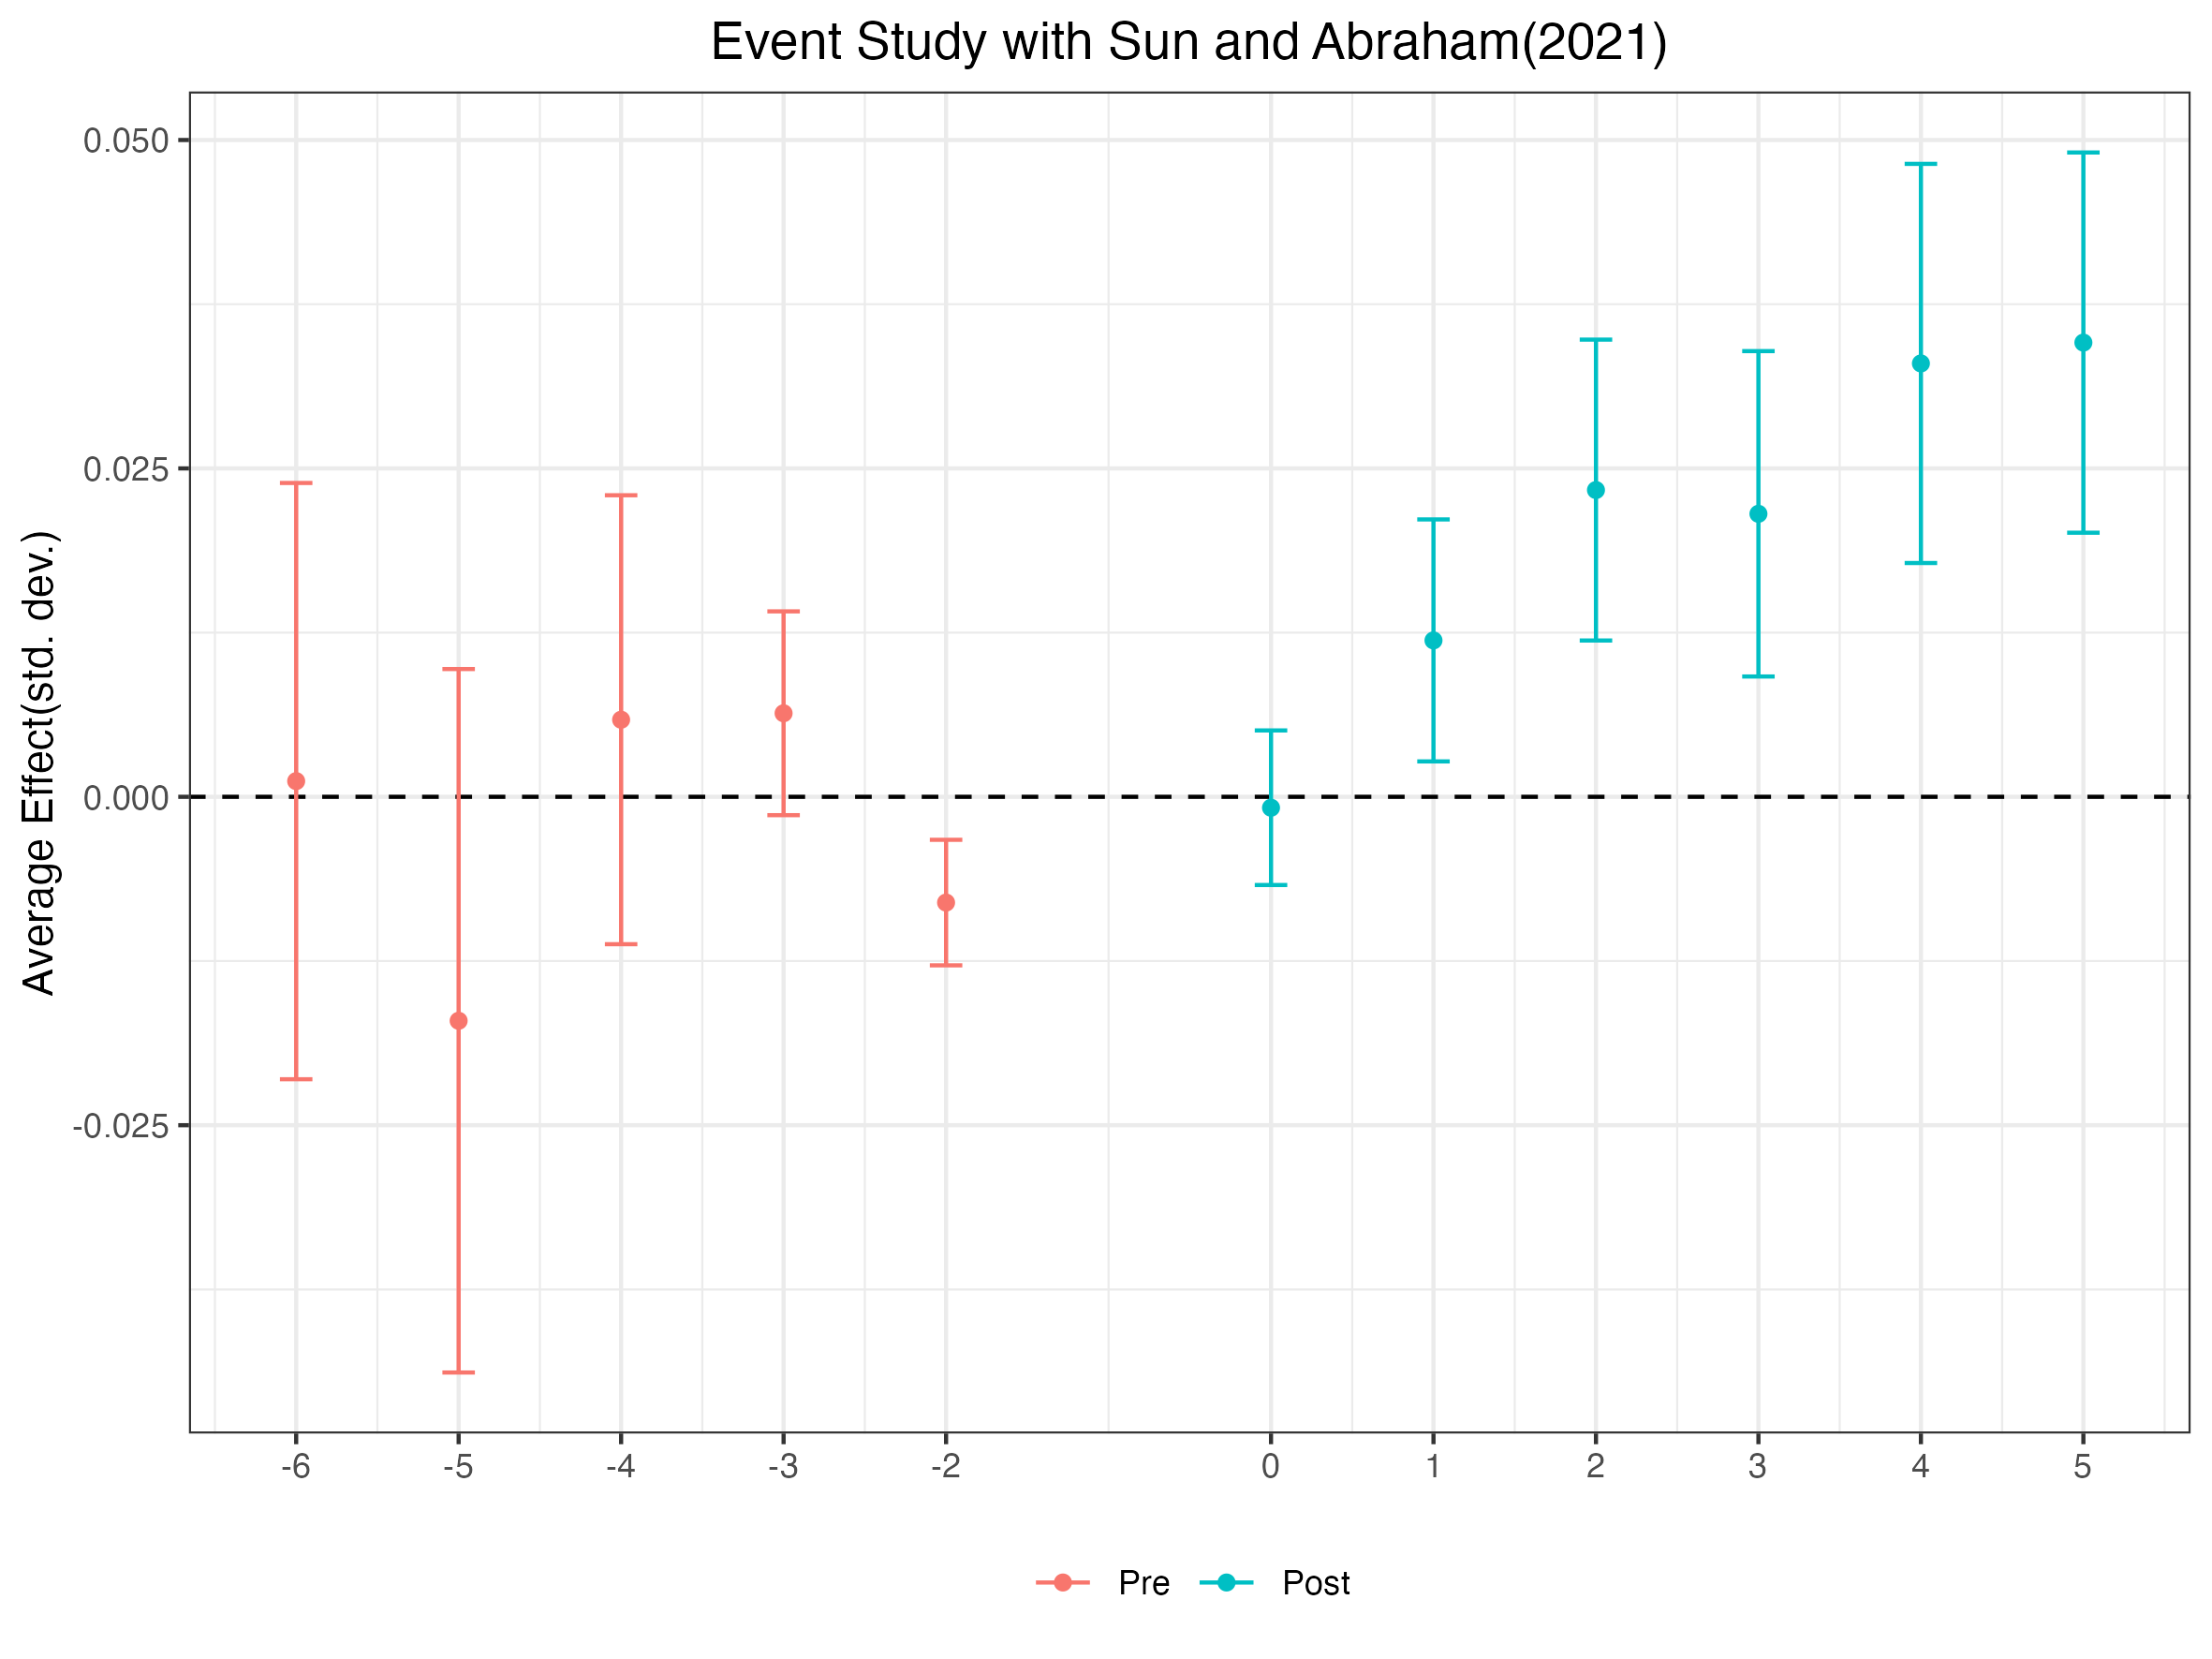
\includegraphics[width=0.6\linewidth, height=4.5cm]{figures/did-base/sadid(logFTOTINC).png}
            \caption{Overall Income}
            \label{fig:Overall Income}
        \end{figure}
    }

    % Frame 1.2: Income by Quartile
    \only<2>{
        \begin{figure}[htbp]
            \centering
            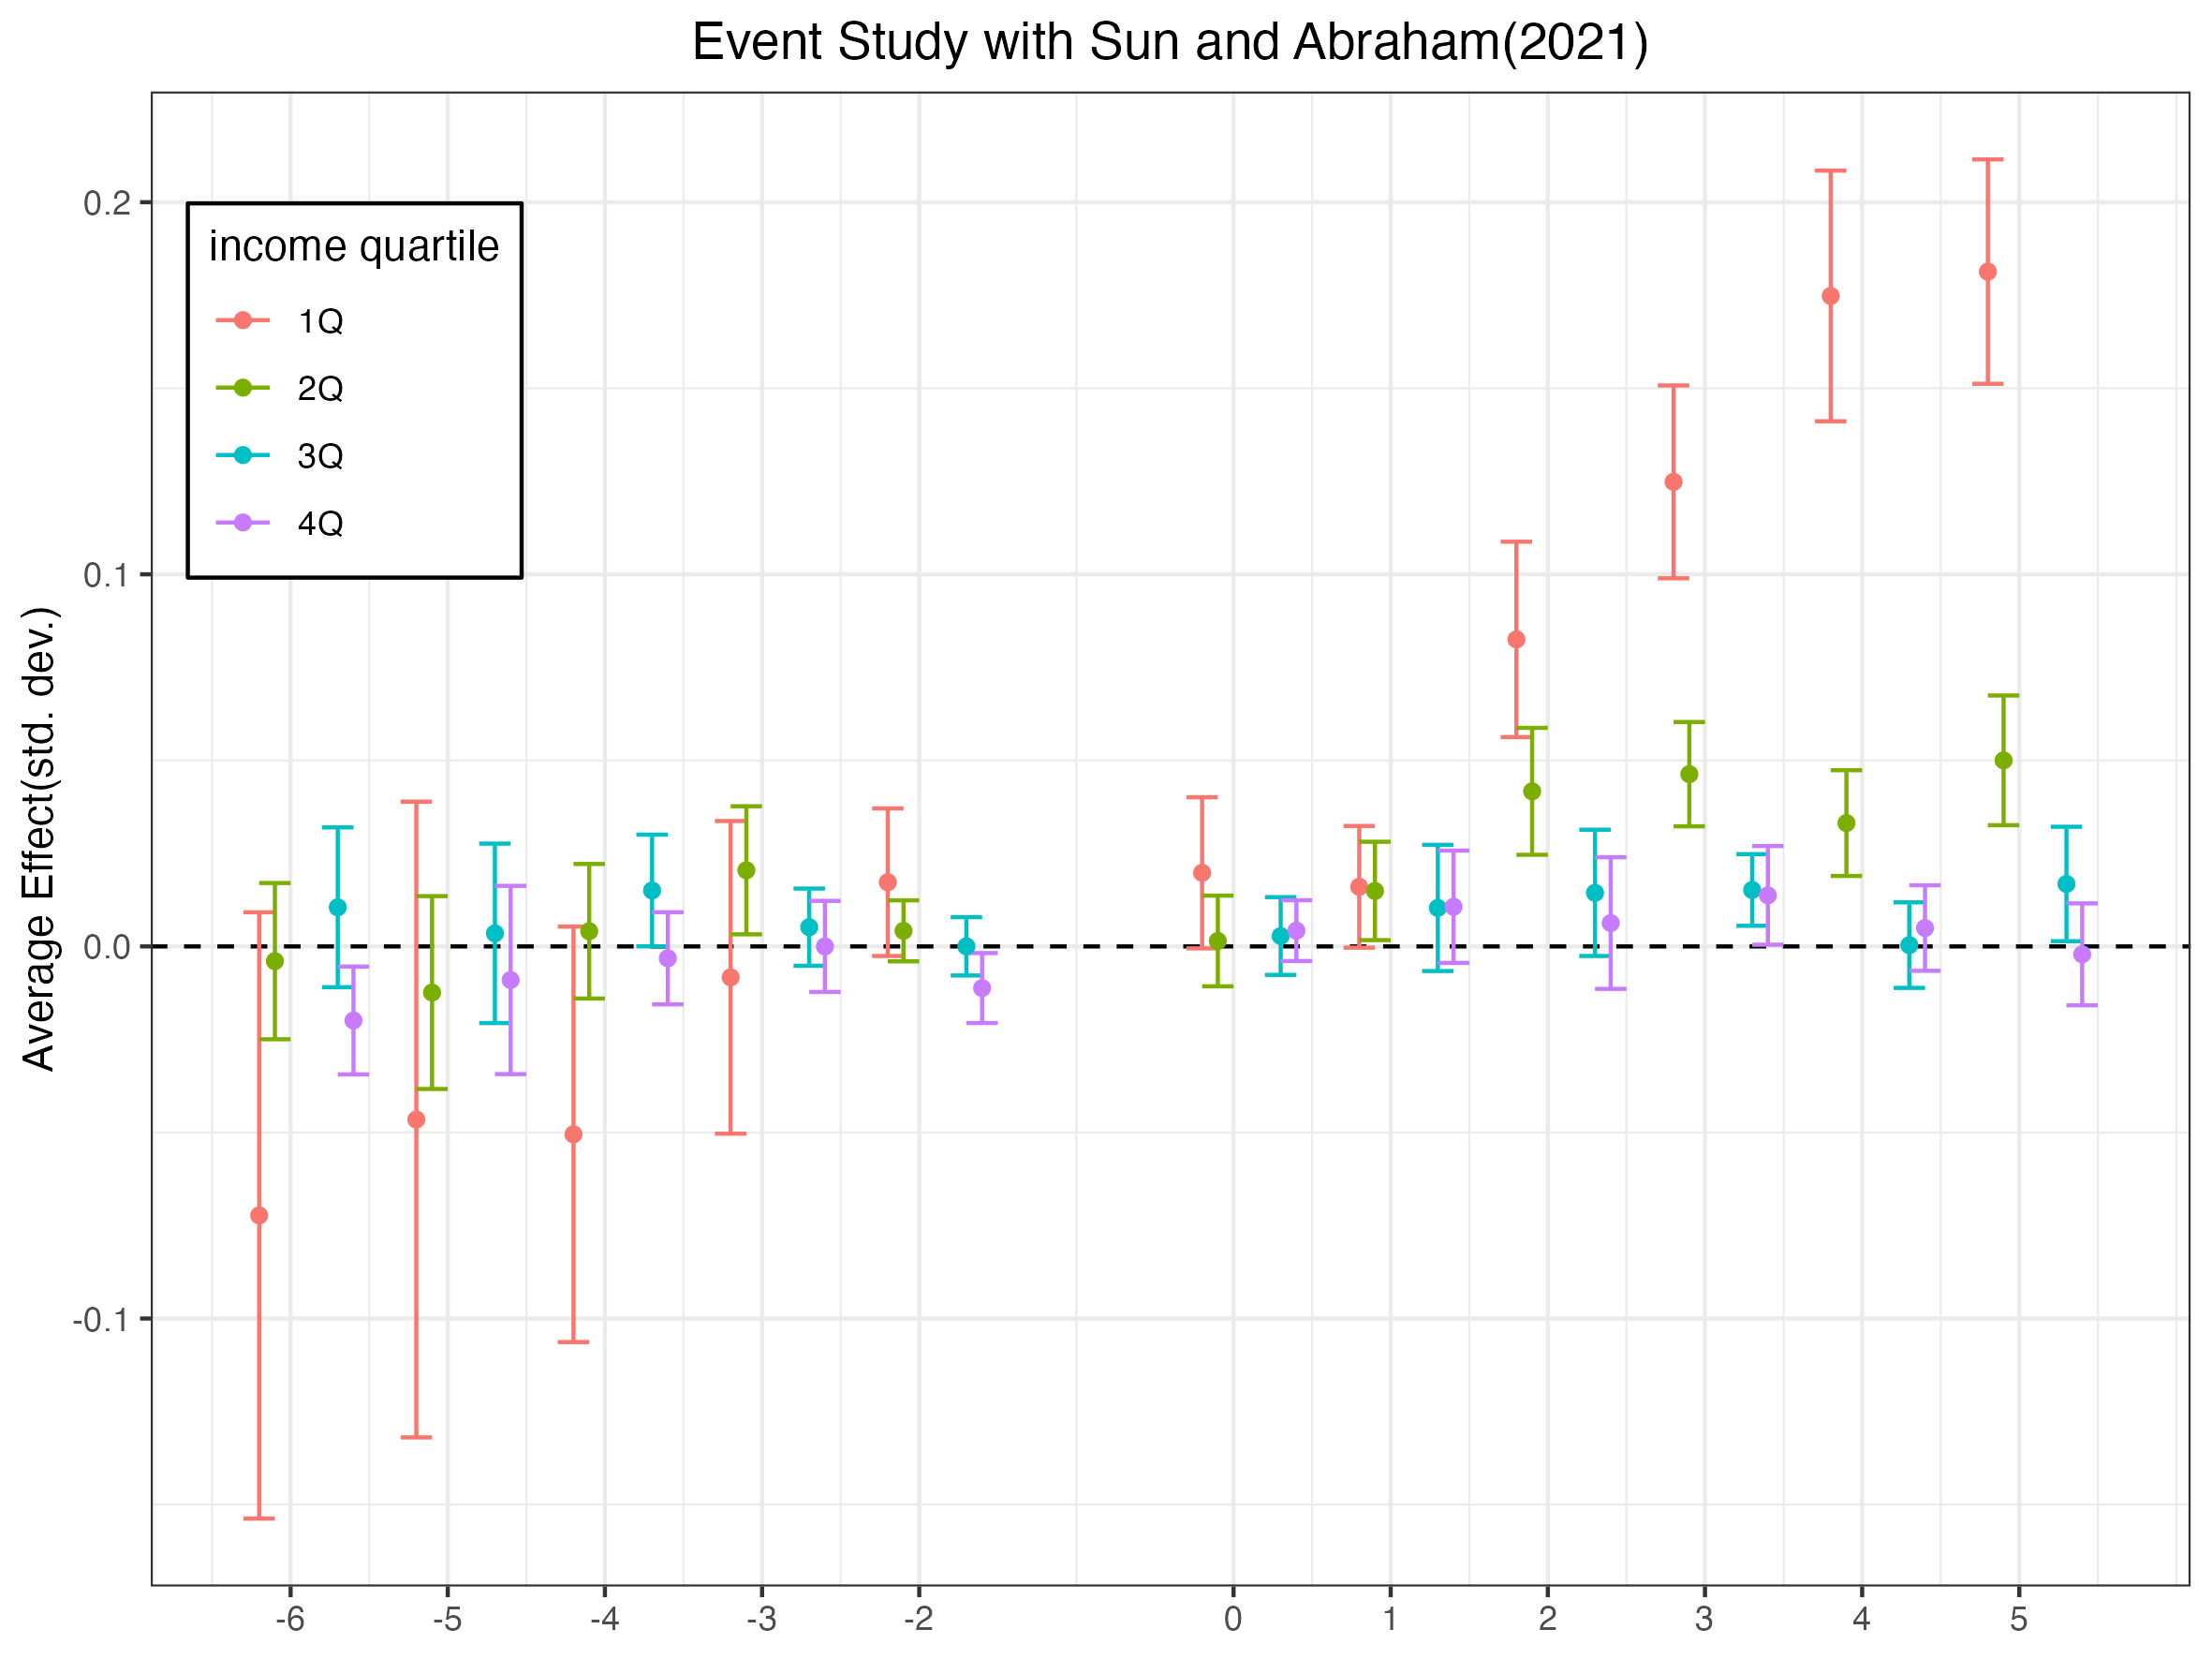
\includegraphics[width=0.6\linewidth, height=4.5cm]{figures/did-base/sadid(logINCTOT - by income quartile).png}
            \caption{Income by Quartile}
            \label{fig:Income by Quartile}
        \end{figure}
    }
\end{frame}
%------------------------------------------------
\begin{frame}{Main Result: Highschool Attendance}
    \vfill
    \begin{itemize}
        \item Highschool attendance decreased by 0.8\% overall in the third year after the shale boom.
        \item increase in 1Q households(18\%)
    \end{itemize}

    % Frame 2.1: High School Attendance
    \only<1>{
        \begin{figure}[htbp]
            \centering
            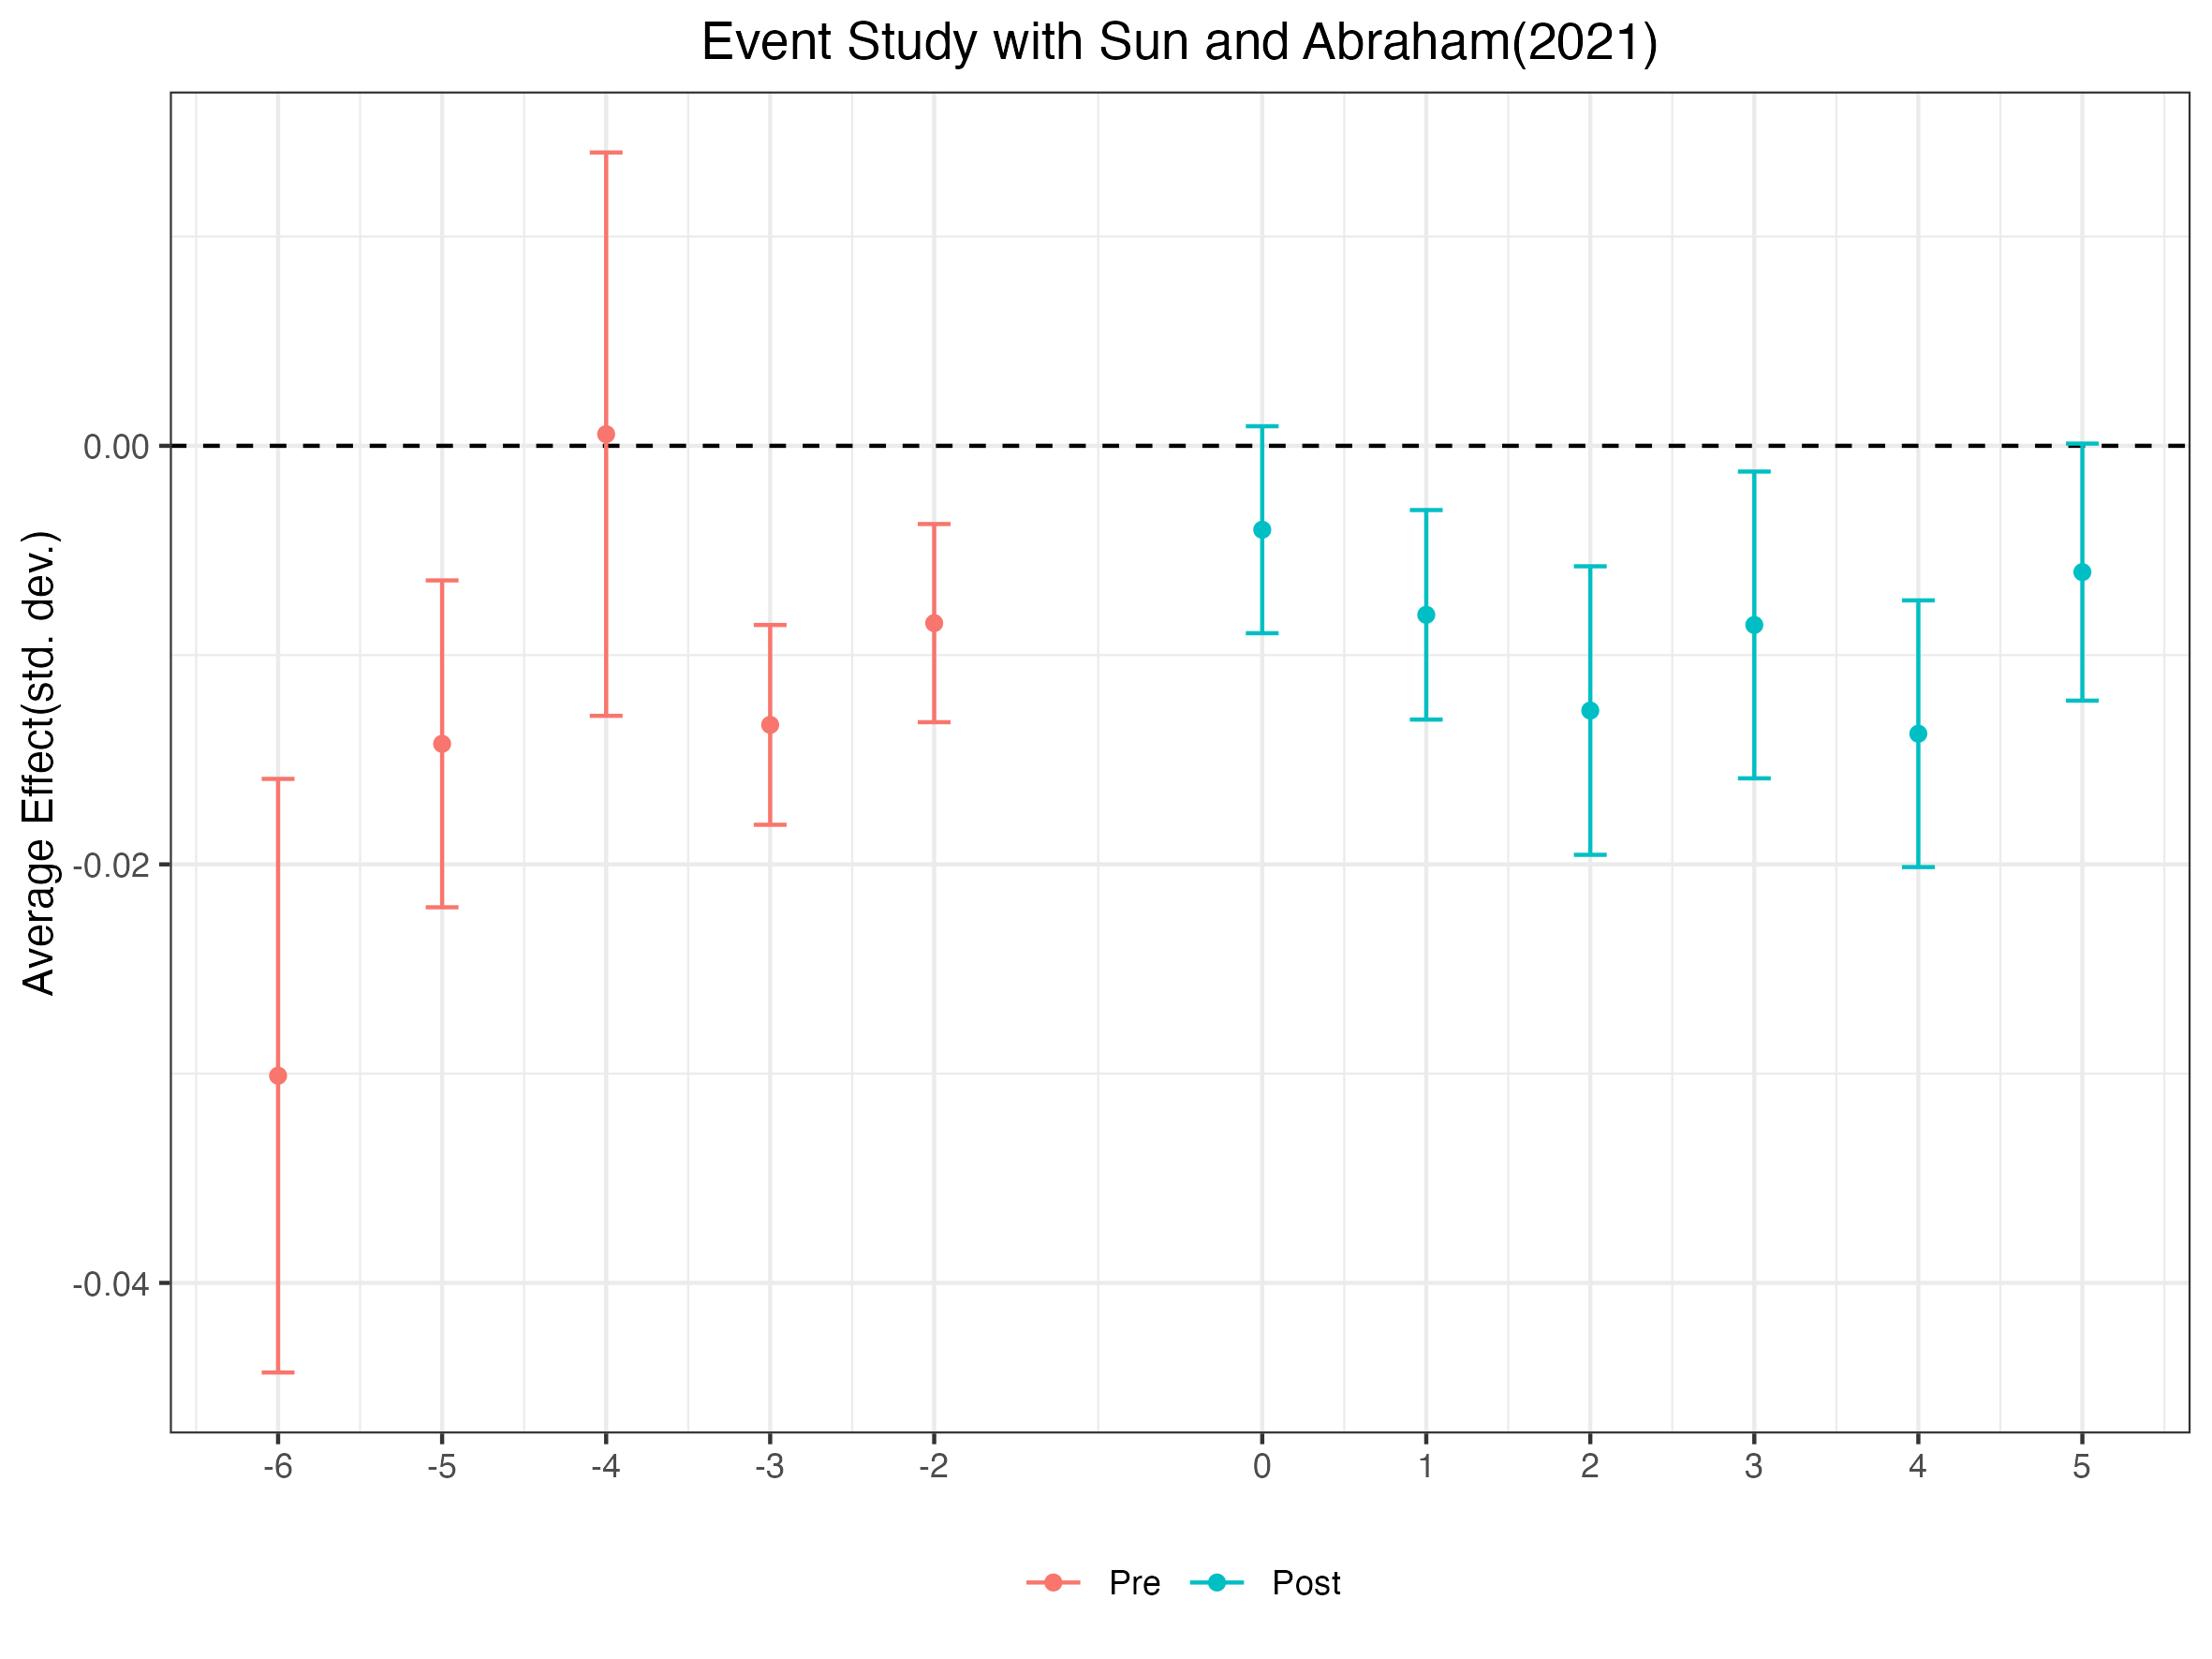
\includegraphics[width=0.6\linewidth, height=4.5cm]{figures/did-base/sadid(high school attendance).png}
            \caption{Highschool Attendance (Overall)} % Adjusted caption for clarity
            \label{fig:hs attendance}
        \end{figure}
    }

    % Frame 2.2: High School Attendance by Quartile
    \only<2>{
        \begin{figure}[htbp]
            \centering
            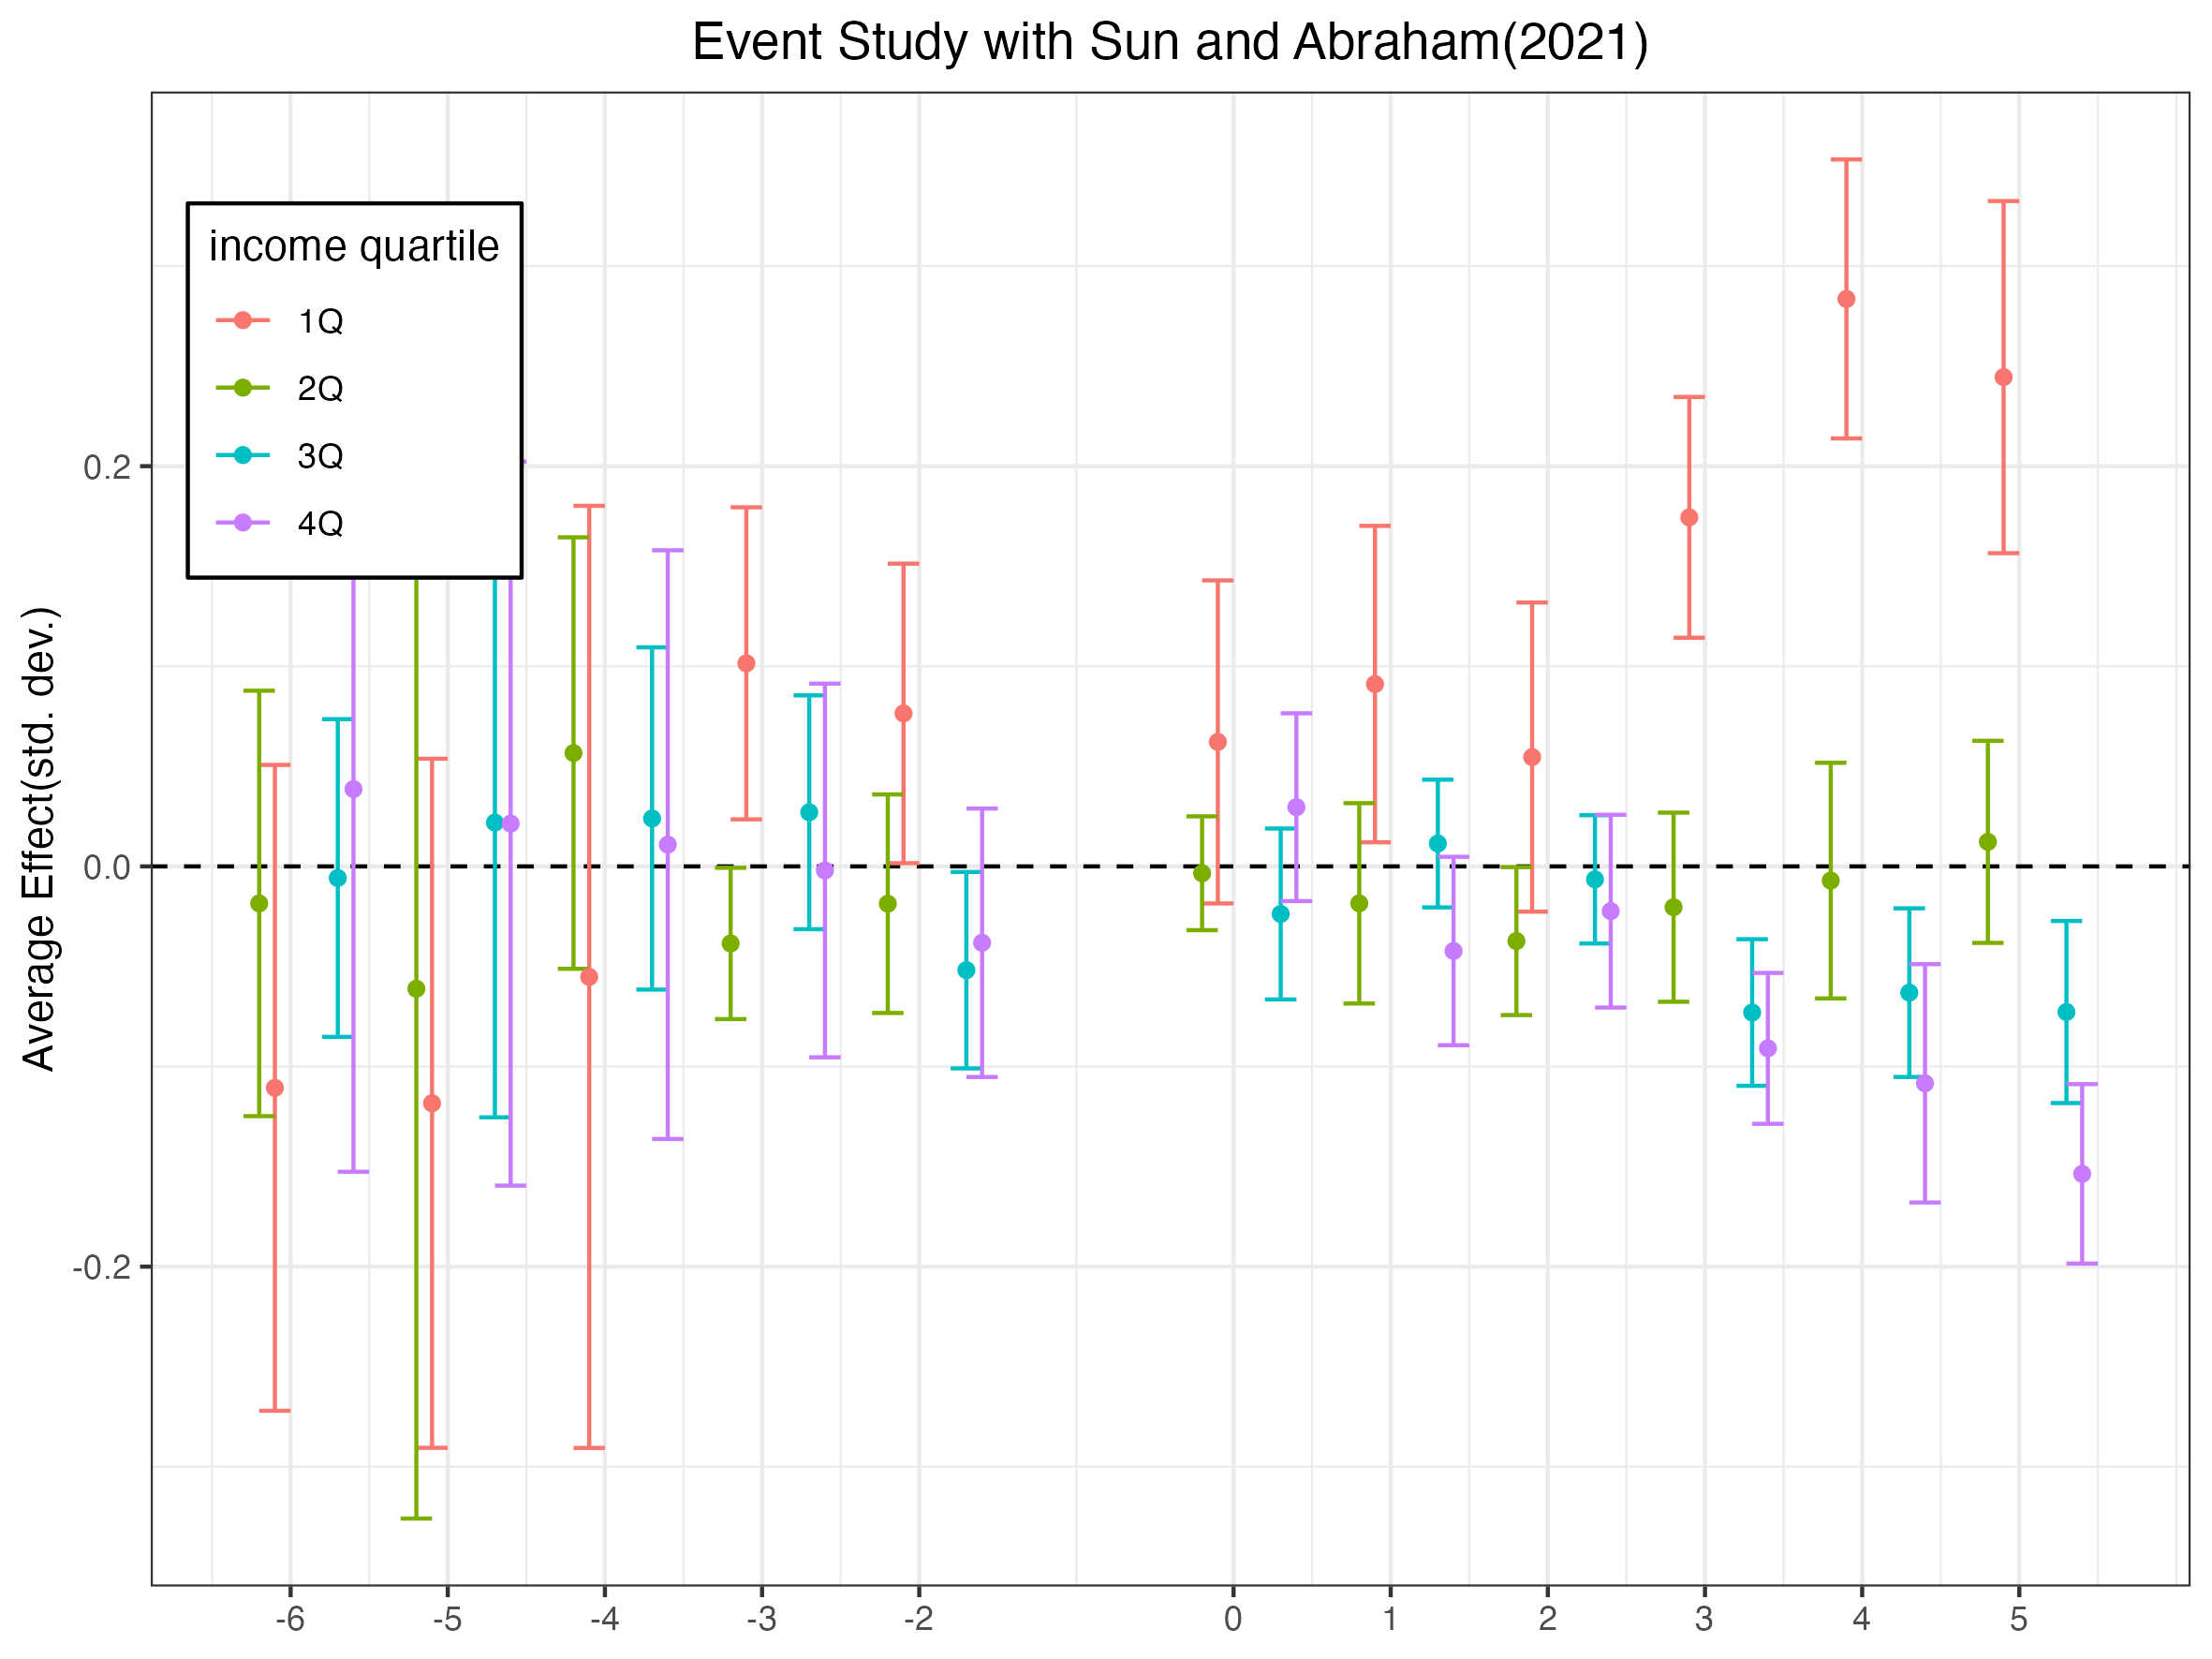
\includegraphics[width=0.6\linewidth, height=4.5cm]{figures/did-base/sadid(high school attendance- by income quartile).png}
            \caption{Highschool Attendance by Income Quartile}
            \label{fig:college shares}
        \end{figure}
    }
\end{frame}

%------------------------------------------------
\begin{frame}{Main Result: College Enrollment}
    \vfill
    \begin{itemize}
        \item College enrollment increased by 7.5\%p overall in the third year after the shale boom.
        \item increase in 1Q households(4.8\%p)

    \end{itemize}

    % Frame 3.1: College Enrollment
    \only<1>{
        \begin{figure}[htbp]
            \centering
            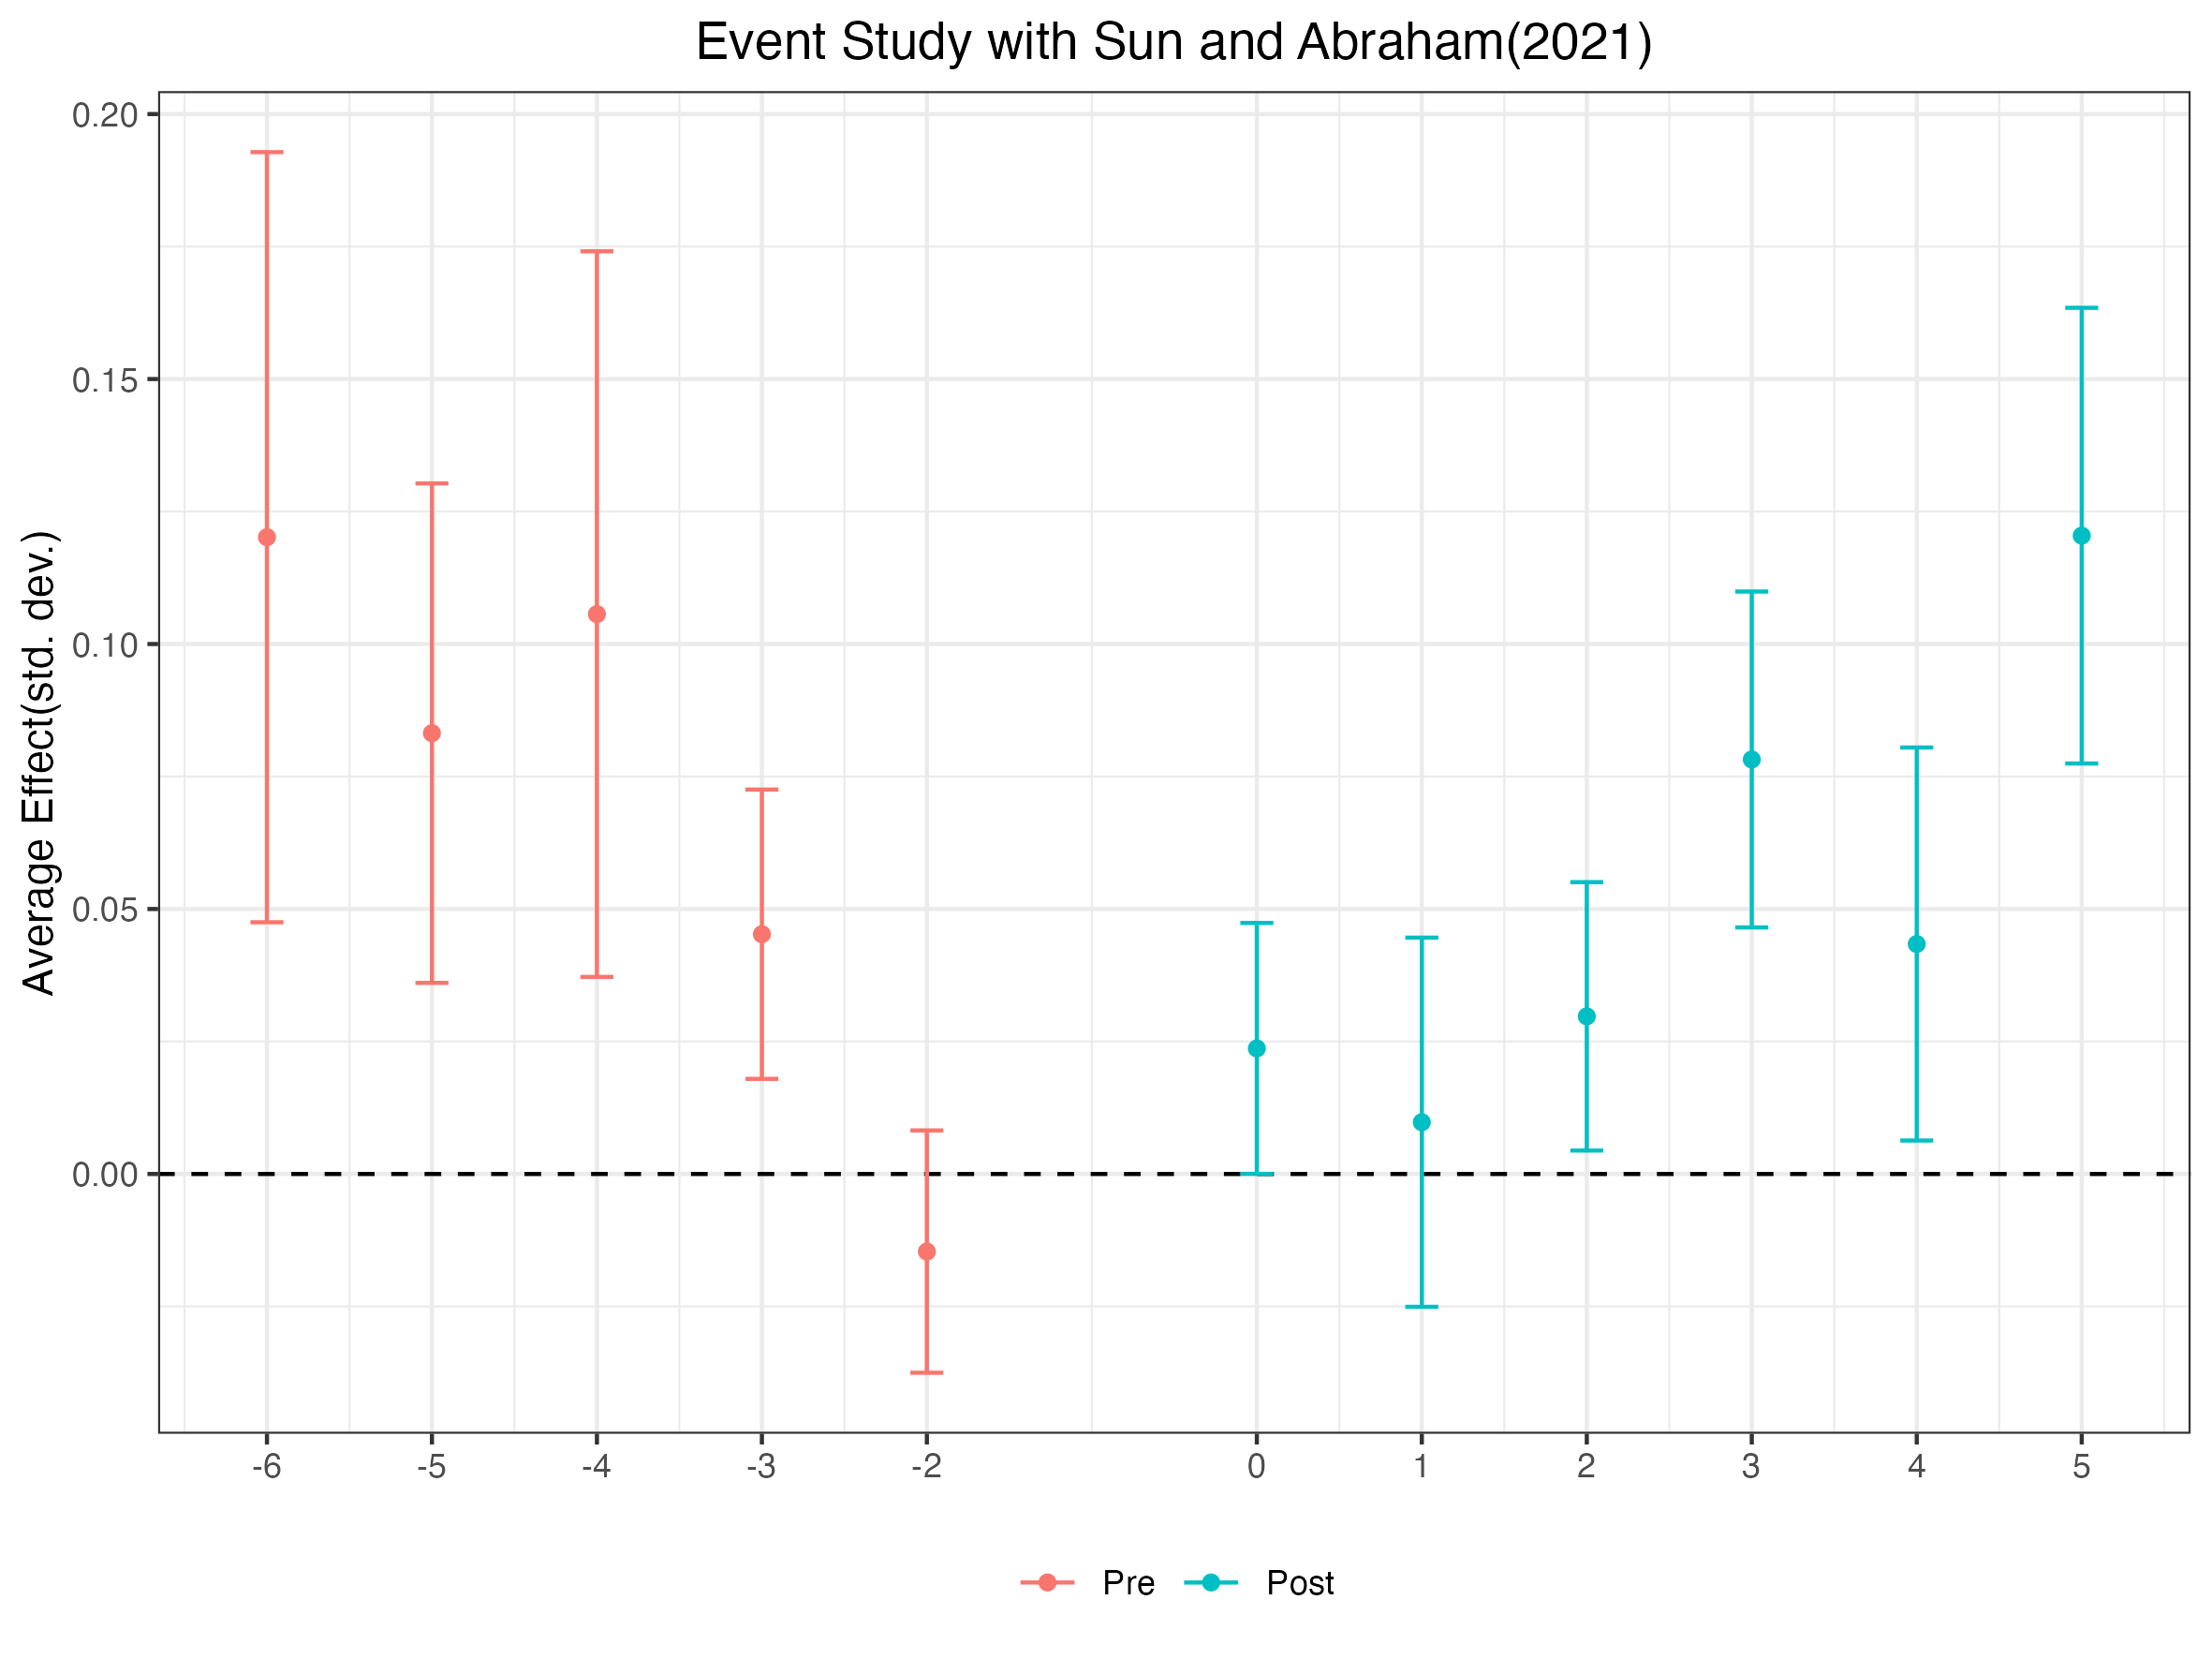
\includegraphics[width=0.6\linewidth, height=4.5cm]{figures/did-base/sadid(college enrollment).png}
            \caption{College Enrollment (Overall)} % Adjusted caption for clarity
            \label{fig:college enrollment}
        \end{figure}
    }

    % Frame 3.2: College Share by Quartile
    \only<2>{
        \begin{figure}[htbp]
            \centering
            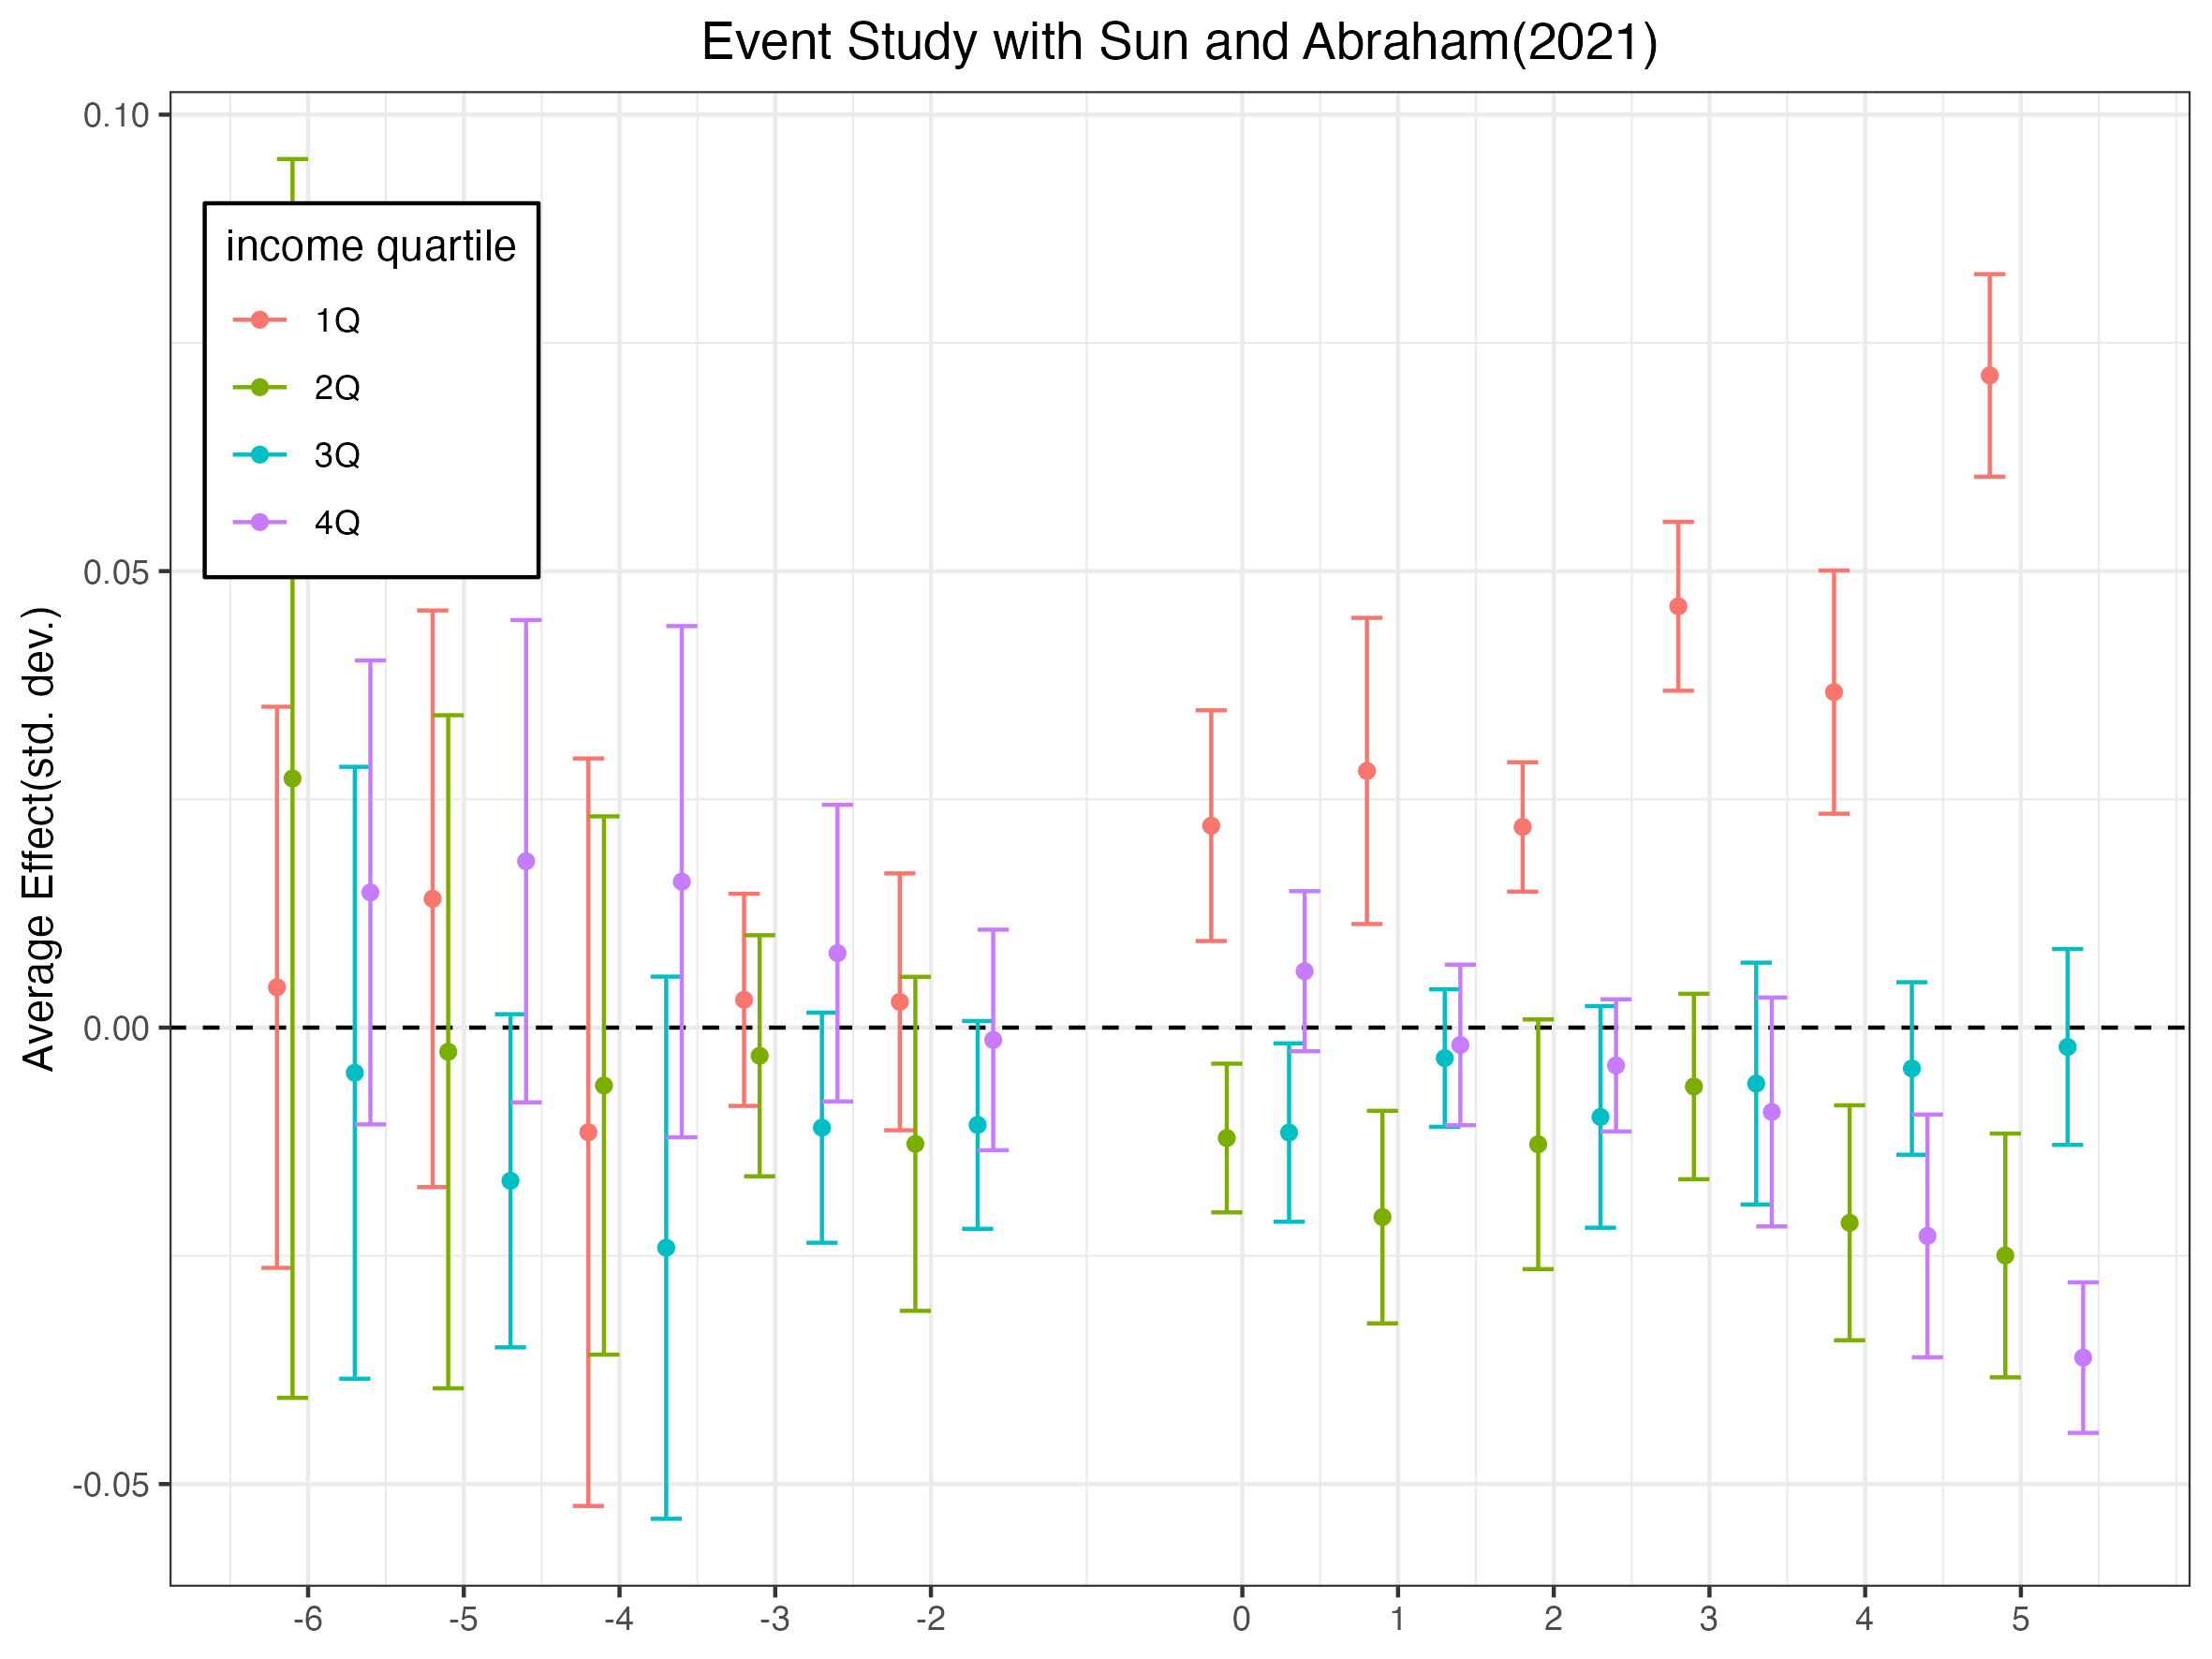
\includegraphics[width=0.6\linewidth, height=4.5cm]{figures/did-base/sadid(college share - by income quartile).png}
            \caption{College Share by Income Quartile}
            \label{fig:college shares}
        \end{figure}
    }
\end{frame}
%------------------------------------------------




\begin{frame}{Validity of the Identification Assumptions}
\label{sec:validity}
\textbf{Parallel Trends}
\begin{itemize}
  \item Some evidence of pre-trends and non-linearity:
    \begin{itemize}
      \item Household income (1Q): slight upward pre-trend, but post-treatment increase is larger and steeper.
      \item hs attendance and college enrollment: significant pre-trend, but disappears when controlling for income $\Rightarrow$ supports \textit{conditional} parallel trends.
    \end{itemize}
  \item Solutions: \textcite{athey2025triply}, \textcite{athey2021matrix}, \textcite{arkhangelsky2021synthetic}
\end{itemize}

\textbf{Compositional Changes}
\begin{itemize}
  \item Concern: selective migration from non-shale to shale states may bias estimates upward.
  \item Evidence: slight increase in migration rate post-treatment, but unclear if this causes bias.\hyperlink{sec:migration}{\beamergotobutton{Details}}
\end{itemize}

\vspace{0.2cm}
\textbf{Dynamic Treatment Effect Homogeneity}
\begin{itemize}
  \item Important assumption for SADiD; discussed further in the analysis.
\end{itemize}
\end{frame}
%------------------------------------------------


\section{Conclusion and Next Steps}
\begin{frame}{Conclusion}

Shale gas boom increased income and college enrollment, especially for low-income households, casting a doubt on the conventional wisdom of the ``Dutch Disease".  But I haven't figured out why. 
    \begin{itemize}
        \item Previous studies reporting an increase in income and a decrease in education are consistent with the traditional trade theory and the \textit{Dutch disease} hypothesis, but we cannot explain why income and education are moving together
        \item \textbf{Next Step(1): }Investigating which students stayed in school, and which students dropped out, will guide us on the characteristics that lead to different decisions.
    \end{itemize}

\end{frame}
%------------------------------------------------
\begin{frame}{Next Steps(2)}
\label{sec:nextstep2}
 \only<1>{Choosing income quartiles for HTE analysis is an arbitrary setup(\cite{athey2016recursive}). Why do we divide the sample by their household income, and why four?}

\onslide<2->{
\begin{itemize}
    \item How can we incorporate ML methods such as causal forest to this research?
    \begin{itemize}
        \item \textcite{wang2024longbet} proposes the following method to estimate CATT in panel data settings:
        \item Outcome Model 
        \begin{align*}
            Y_{it} = \alpha \mu(X_i, T = t) + \beta_S \nu(X_i, S_{it},T = t) + \epsilon_{it}
        \end{align*}
        where $S$ is the length to exposure (Train XBART forests separately for $\mu$ and $\nu$)
        \item CATT: \begin{align*}
            \tau_t(X_i, S) &\equiv  \mathbb{E}[Y_{it} | X_i, S_{it} = S] - \mathbb{E}[Y_{it} | X_i, S_{it} = 0] \\
            &= \beta_S \nu(X_i, S_{it}, T = t) - \beta_0 \nu(X_i, S=0, T = t)
        \end{align*}
    \end{itemize}
    \item Drawback: a type of T-learner, which has known problems identifying CATTs(e.g. regularization bias)\hyperlink{sec:regbias}{\beamergotobutton{Example}}
\end{itemize}
}


\end{frame}
%------------------------------------------------
\begin{frame}{Next Steps(2)}

\footnotesize

The ideal solution in the metalearner literature is to use the\textbf{ R-learner}(\cite{kunzel2019metalearners}, \cite{chernozhukov2022locally}): $\sqrt{n}$-consistent and follows the CLT under reasonable limits
\begin{align}
Y_i &= \mu_(0)(X_i) + W_i \tau(X_i) + \varepsilon_i\\
&=m(X_i) + (W_i-e(X_i))\tau(X_i) + \varepsilon_i
\end{align}

where $\mathbb{E}[\varepsilon_i|X_i, W_i]=0$ and 

\begin{align}
    e(x) &= \mathbb{E}[W_i|X_i=x]\\
    m(x) &= \mathbb{E}[Y_i|X_i=x] = \mu_{(0)}(x) + e(x)\tau(x)
\end{align}

which allows the following \textit{residuals-on-residuals}

$$
Y_i - m(X_i) = \bigl(W_i-e(X_i)\bigr)\tau(X_i) +\varepsilon_i
$$

\end{frame}
%------------------------------------------------

\begin{frame}{Next Steps(2)}

DGP for the Panel Case(with mostly the same assumptions as in \textcite{sun_estimating_2021})
\begin{align}
Y_{it}(S) &\perp <D_{i1}, D_{i2}, \dots, D_{iT}> | X_i \qquad \forall S=0, 1, \dots T\\
Y_{it} &= \sum_{s=1}^T \mathbb{I}(S_{it} = s)\tau(X_i,s) + g_0(X_i, \delta_t) + \varepsilon_{it} \label{eq:rlearner-panel} \\
D_{it} &= m_o(X_i) + \nu_{it}
\end{align}

where $\varepsilon$ and $\nu$ satisfies $\mathbb{E}[\varepsilon |D,  X] = 0$ and $\mathbb{E}[\nu | X] = 0$.

Equation (\ref{eq:rlearner-panel}) implies that for untreated individuals and periods,

$$
Y_{it} - Y_{it'} = g_0(X_i, \delta_t) - g_0(X_i, \delta_t') \qquad \forall t \neq t'
$$

\end{frame}


\begin{frame}
    \centering
    \vfill % Pushes content down
    
    \Huge \textbf{Thank You:)} 


    \vfill % Pulls content up

\end{frame}

%----------------------------------------------------------------------------------------
\section*{Appendix}
\begin{frame}{Appendix}
\label{sec:migration}
\begin{figure}[htbp]
    \centering
    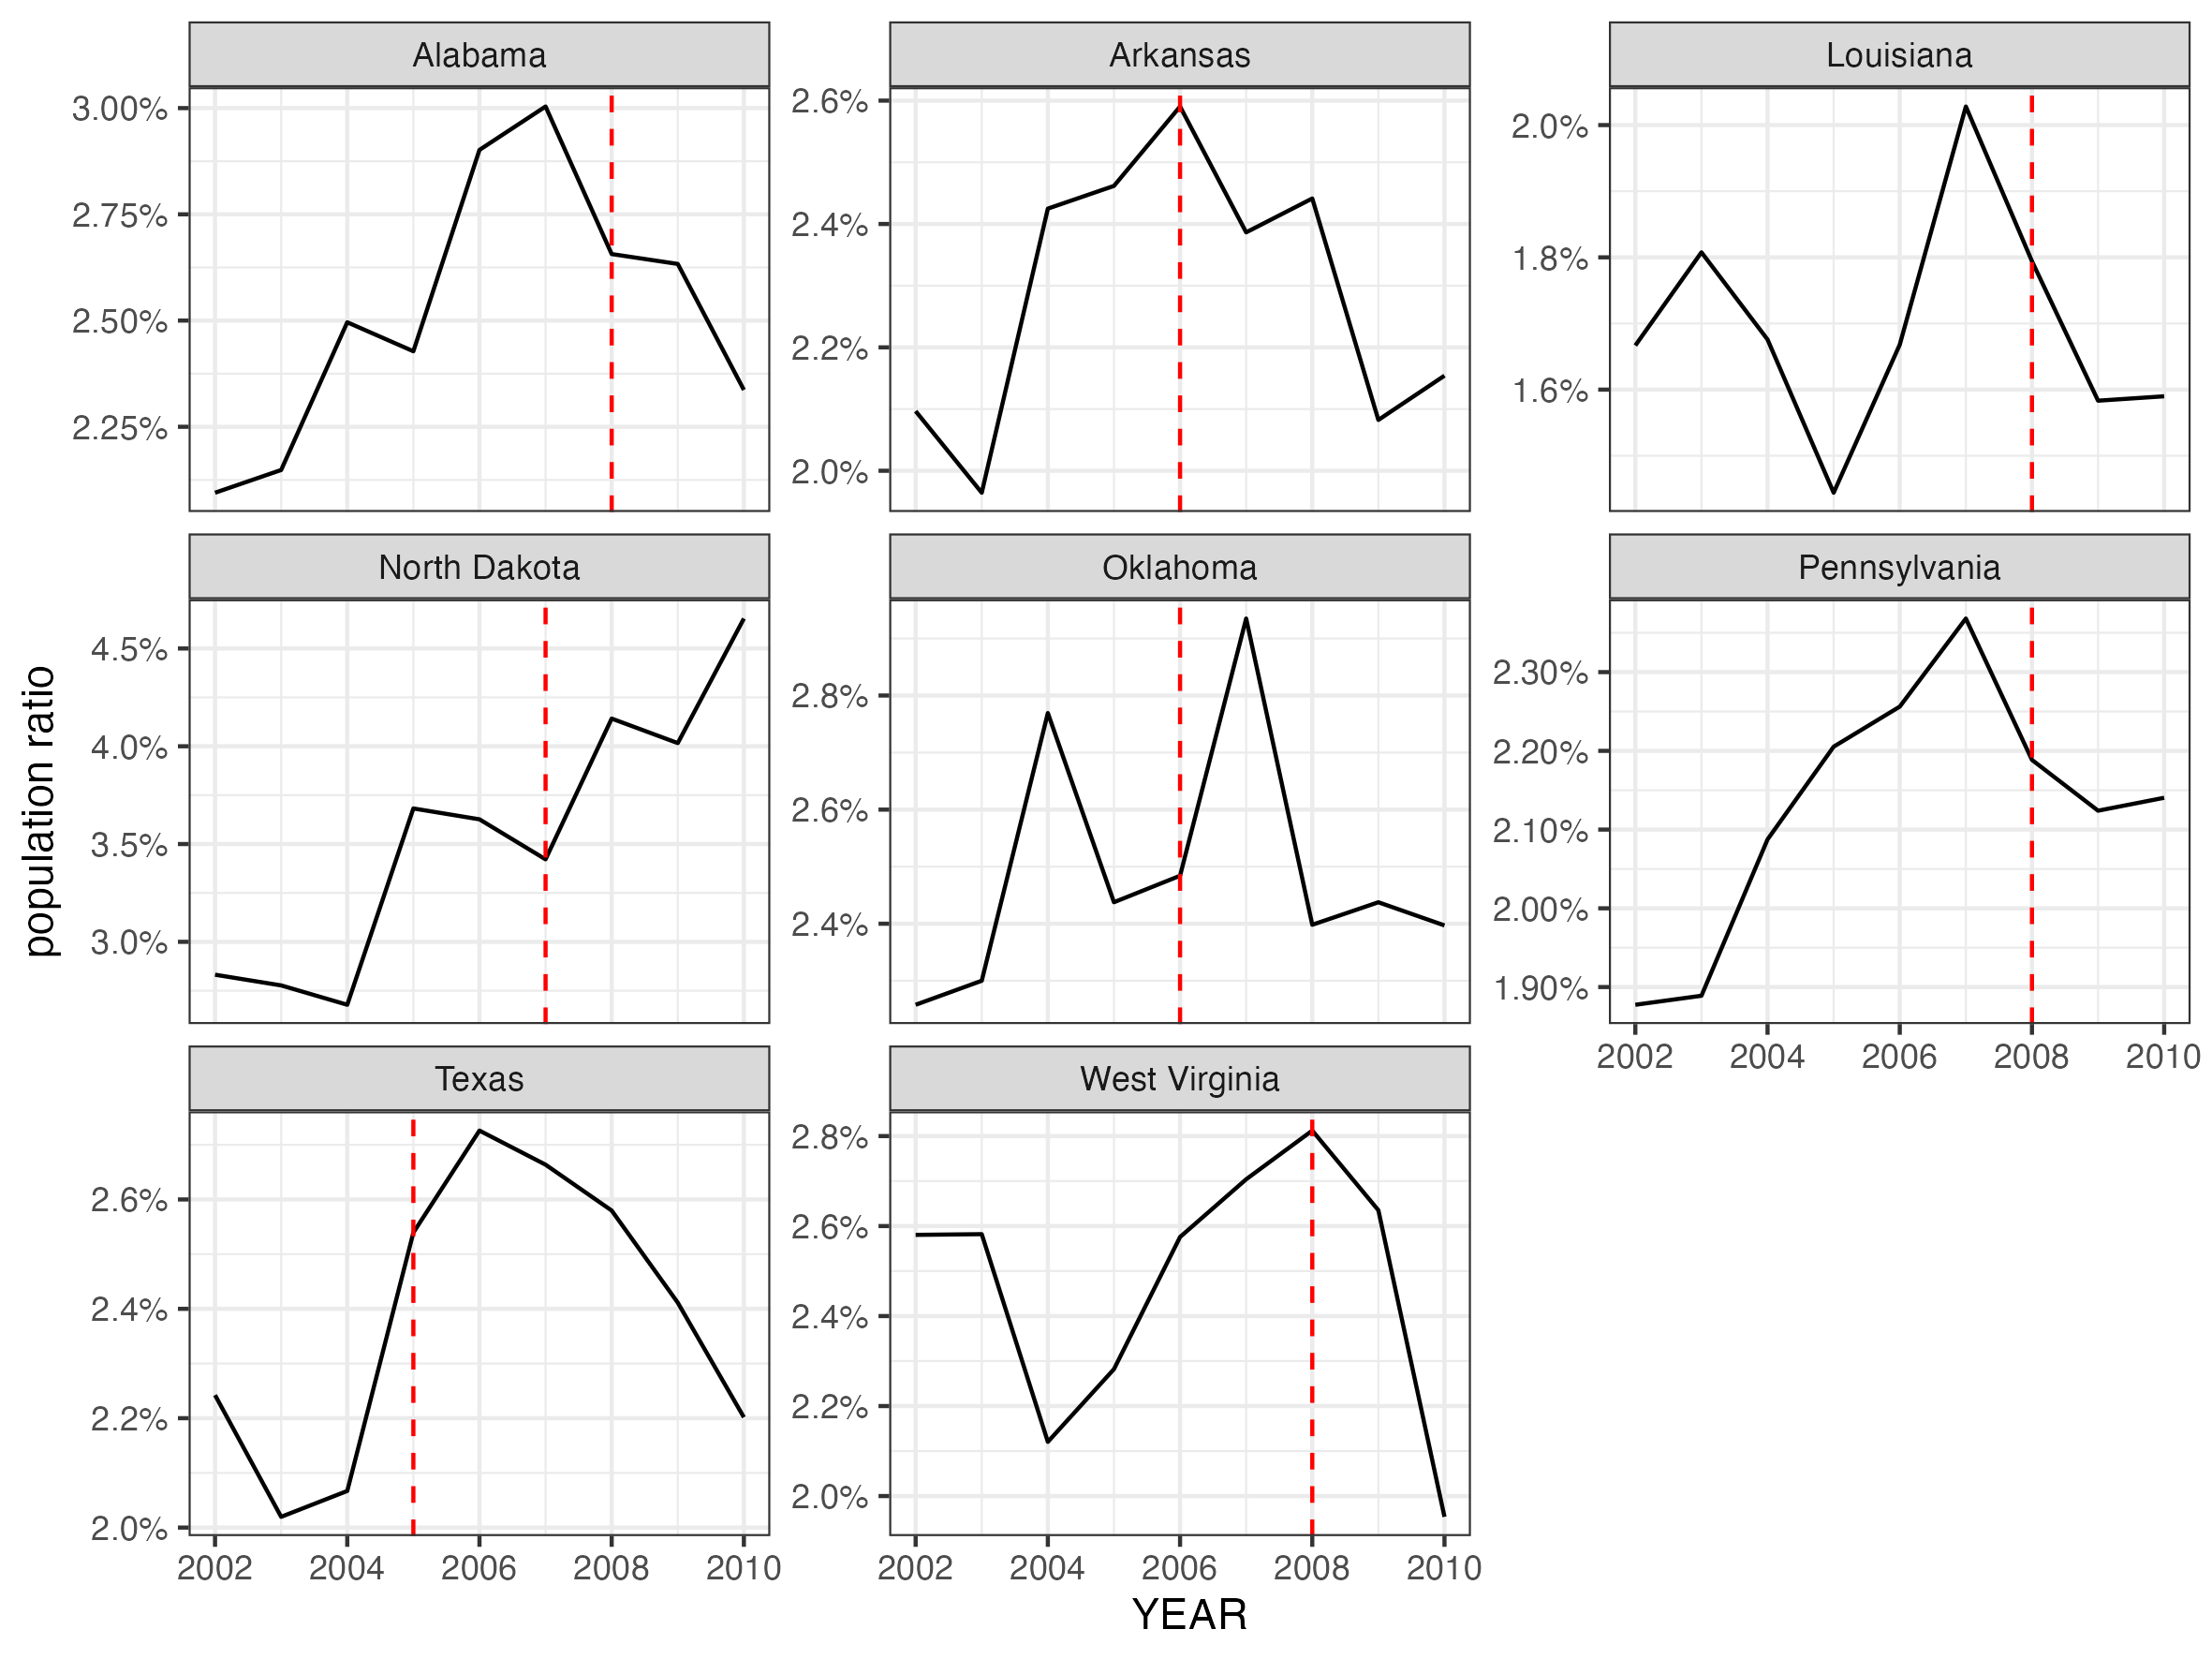
\includegraphics[width=0.5\textwidth]{figures/pop_ratio_from_outside.png}
    \caption{Migration Rate Before and After the Shale Gas Shock}
    \label{fig:migration}
\end{figure}
\raggedleft
\hyperlink{sec:validity}{\beamerreturnbutton{return}}
\end{frame}



\begin{frame}{Appendix}
\label{sec:regbias}
\begin{figure}[htbp]
    \centering
    
\includegraphics[width=0.5\textwidth]{doc/figures/reg-bias-example.png}
    \caption{Example from \textcite{kunzel2019metalearners} on T-learners}
    \label{fig:reg-bias}
\end{figure}
\raggedleft
\hyperlink{sec:nextstep2}{\beamerreturnbutton{return}}
\end{frame}


\begin{frame}{References}
\tiny
\printbibliography[heading=none]
\end{frame}

\end{document}
